\documentclass{source/Paper}
\usepackage{tabularx}
\usepackage{subcaption}
\usepackage{float}
% \usepackage{gbt7714}
\usepackage{subfigure}
\usepackage{enumitem}
\usepackage[backend=biber, doi = false, citestyle=gb7714-2015, bibstyle=gb7714-2015]{biblatex}
\usepackage{cleveref}
\lhead{新时期``容貌焦虑''在大学生群体中的表现及影响研究报告——以大一学生为例}
\addbibresource{ref.bib}
\articletitle{新时期``容貌焦虑''在大学生群体中的表现及影响研究报告}
\name{欢乐斗地组}
\date{\today}
\stuid{}
\Abstract{
本研究对现代社会一个不可忽视的心理健康问题——``容貌焦虑''在当代大学生群体中的存在现状展开研究,
阐述医美、社交媒体和广告文化与大学生``容貌焦虑''之间的关系以及``容貌焦虑''对大学生心理和社交行为产生的影响,
并提出了缓解容貌焦虑的可能路径。
}
\Keyword{大学生;容貌焦虑;容貌;心理健康}
\begin{document}
\thispagestyle{empty}

\vfill

\begin{center}
    
\includegraphics[width=0.5\paperwidth]{./source/logo/zjuchar.pdf}
\end{center}

\begin{center}
    \zihao{-1} \heiti \bfseries
    研~究~性~学~习~研~究~报~告
\end{center}

\vskip 20pt

\begin{center}
    
\includegraphics[width=0.17\paperwidth]{./source/logo/zju.pdf}
\end{center}

\vskip 20pt
\begin{center}
    \bfseries \zihao{3}
    \begin{tabularx}{.7\textwidth}{>{\fangsong}l >{\fangsong}X<{\centering}}
        \fangsong
        题目      &  \underline{\hfill 新时期``容貌焦虑'' \hfill} \\
        ~        & \underline{\hfill 在大学生群体中的表现及影响研究报告 \hfill} \\
        小组名称 & \underline{\hfill 欢乐斗地组 \hfill} \\
        组长& \underline{\hfill 郭慧婷 \hfill} \\
        小组成员 & \underline{\hfill 何铭源、蒋子墨、阎乐暄、诸葛一涵 \hfill} \\
        ~ & \underline{\hfill 江善钊、任弈、赵皓翌、余文乐 \hfill} \\

    \end{tabularx}
\end{center}
\vfill
% \makeheader
\setcounter{page}{0}
\newpage
\tableofcontents
\newpage
\makeheader

\noindent\rule{\textwidth}{1pt}

\section{研究背景及现状}
\subsection{研究背景}
容貌焦虑已成为现代社会一个不可忽视的心理健康问题,尤其在年轻群体中表现得尤为突出。
随着科技的进步和社交媒体的普及,人们对外貌的关注度日益增加。
这种焦虑不仅影响个人的心理健康,还可能对他们的社交、工作和生活产生负面影响。

近年来,多项研究调查揭示了容貌焦虑的普遍性。
例如,2021年中青校媒面向全国2063名高校学生进行的容貌焦虑话题调查显示,59.03\%的大学生存在一定程度的容貌焦虑。
这一数据表明,容貌焦虑已经成为大学生群体中一个值得关注的现象。
此外,社交媒体和互联网技术的发展,使得``标准美''的形象被广泛传播和推崇,进一步加剧了年轻人的外貌压力。

容貌焦虑的形成原因是多方面的。
主观心理因素如自卑、敏感和攀比心理是引发容貌焦虑的重要原因。
客观环境因素同样对容貌焦虑的产生起到了推波助澜的作用。社会规范和大众传媒所构建的``大众审美''标准,对个体产生了深远的影响。
职场中的``颜值经济''现象也加剧了容貌焦虑,一些行业和岗位对外貌有着较高的要求,使得外貌成为了评价个人能力和价值的一个标准。

容貌焦虑的研究不仅有助于深入了解这一现象的成因和影响,还能为个体提供有效的应对策略,帮助他们建立正确的自我认知和健康的审美观念。通过心理健康教育和社会支持,可以减轻容貌焦虑对年轻人的负面影响,促进他们的心理健康和全面发展。

\subsection{研究现状}
\subsubsection{陈雪莹}
陈雪莹采用问卷调查法和统计分析法,对大学生群体使用抖音短视频平台引发的容貌焦虑加速现象进行分析,发现理想美内化在抖音使用强度与容貌焦虑的影响路径中发挥中介作用,上行社会比较发挥调节作用。
并据此提出减少大学生容貌焦虑的有效建议,以纠正当前抖音使用对大学生群体产生的审美观念扭曲问题。\autocite{__2022-3}

但是该论文存在局限性:研究对象仅局限于抖音用户中的大学生,样本具有一定的局限性,可能无法完全代表所有大学生群体。此外,对于容貌焦虑的测量和评估可能存在一定的主观性。


\subsubsection{祝旭冉和尹升志}
祝旭冉和尹升志采用量表设计、问卷发放、深度访谈,提出了
容貌焦虑的诱因:引起大学生容貌焦虑的具体原因有身材不好、单眼皮、脸上有痣、脱发等。
大学生群体在容貌焦虑的认知、态度、行为3个方面之间极易出现失衡现象。
其中心理原因、他人评价和审美观念的普及这三点对于容貌焦虑的产生有很大影响。\autocite{__2023}


\subsubsection{李升和李敏}
李升和李敏分析了容貌焦虑的成因和对应的解决方法:不仅需要从个体层面加强青年心理健康教育和服务,使其形成自尊自信、
理性平和、积极向上的良好心理素质,还需要更多从社会层面关注青年女性``容貌焦虑''的形成机制及结果,通过对社会性别规范更为 面的引导与改善,
在社会层面培育起积极正向的关于 身体的社会价值观与开放包容的审美文化。
同时需要持续优化青年群体的文化环境,构建更为丰富的美育氛围,媒体和网络媒介的内容与传播需有益于青年群体的健康成长,避免消费社会中的身体商品化消费意 识形态侵蚀社会舆论,以此推进在社会中形成整体 性、全面性、积极性的美感文化。\autocite{__2022-2}

还有很多关于分析网络对于青少年容貌焦虑形成的文献\autocite{_sisi_2024}。

\subsubsection{局限性}
这些研究都未深入研究大学生产生容貌焦虑的过程中所受到的诸如社会规训、美容美体广告、新时期一些新思潮在网络上的广泛传播等具体因素的影响。

\subsection{研究目的及意义}

\subsubsection{个体角度}
在个体身心健康和时间管理层面,我们小组希望可以通过此次研究,引导有容貌焦虑的人群悦纳自己,
乐观生活,帮助他们建立包容的、多元的审美价值体系,不被社会价值体系所裹挟,从心出发做自己。

\subsubsection{社会群体}
在美的定义和标准多元化层面,我们小组希望可以通过研究让人们不再为社会审美所束缚,
让``审美多元化''真正深入人们心中,从而对社会平稳运行产生一定积极影响。

\subsection{概念界定}
容貌焦虑是指在放大颜值作用的环境下,很多人对于自己的外貌不够自信,从而产生出自卑、痛苦的心理病症。

容貌焦虑者本身没有容貌绝对缺陷,但总对自身的容貌产生自卑和不满情绪。

而容貌焦虑的具体表现分为三个方面,具体如
图(\ref{pic:juti})所示
\begin{figure}[htbp]
    \centering
    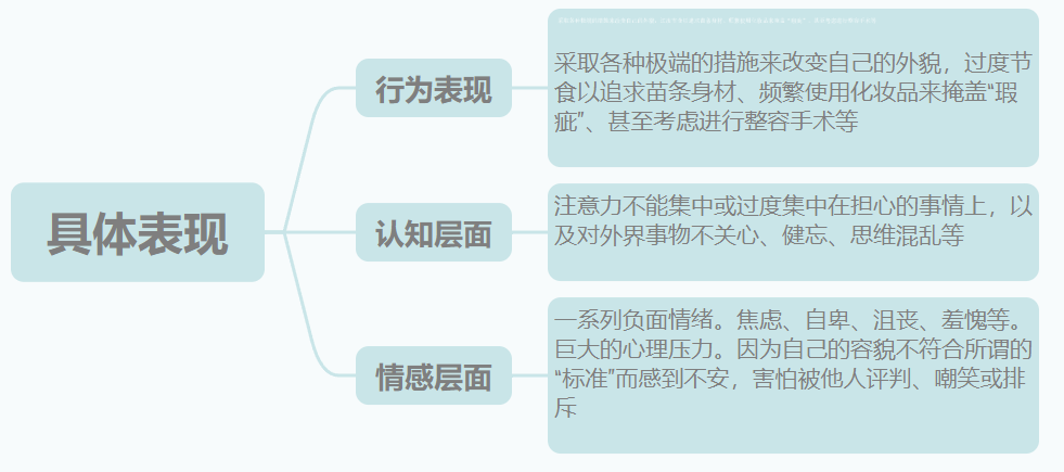
\includegraphics[width=0.7\textwidth]{具体表现.png}
    \caption{容貌焦虑的具体表现}
    \label{pic:juti}
\end{figure}



\section{研究方法}
考虑到本次研究性学习与大学生有着密切联系,所以我们采用了问卷调查的研究方法,并在选取典型样本进行更加细致的采访调查,旨在更好的了解``容貌焦虑''在大学生中的影响情况。
我们还采访了专业的老师,希望从中了解更加专业成熟的想法。
\subsection{查找资料}
在网络上查找相关资料,论文,了解``容貌焦虑''问题的相关信息
\subsection{问卷调查}
通过发放问卷并统计数据,获得关于大学生群体容貌焦虑问题的相关情况
\subsection{采访相关人士}
采访有典型烦恼的同学,以及有经验的老师,来获取解决的方法
\subsection{数据汇总研究}
分析网络上收集的数据,收集的数据,得出结论
\subsection{研究计划}
\begin{table}[H]
    \caption{研究计划时间表}
    \begin{tabularx}{\textwidth}{>{\raggedright\arraybackslash}X
        | >{\raggedright\arraybackslash}X}
    \hline
    \textbf{时间}                                                                             & \textbf{分工}                                                                                                         \\ \hline
    \begin{tabular}[c]{@{}l@{}}\textbf{秋学期第4周}\\ 查找资料\end{tabular}                      & 查找``容貌焦虑''的说法从何而来                                                                                                                    \\ \hline
    \begin{tabular}[c]{@{}l@{}}\textbf{秋学期第5周}\\ 制作问卷\end{tabular}                        & \begin{tabular}[c]{@{}l@{}}调查自认为有``容貌焦虑''和不认为自己有``容貌焦虑'' \\ 的主要群体(以年龄段、审美类型、家庭氛围等进行分类)\\ 调查诱发``容貌焦虑''的社会环境因素(广告、媒体等) \\ 和个人心理因素\end{tabular} \\ \hline
    \begin{tabular}[c]{@{}l@{}}\textbf{秋学期第6、7、8周}\\ 进行采访\end{tabular}                    & \begin{tabular}[c]{@{}l@{}}调查``容貌焦虑''的具体表现和影响 \\ 调查``容貌焦虑''主要集中在总结出来的群体的原因 \\ 调查大学生群体对``容貌焦虑''的认识\end{tabular}                       \\ \hline
    \begin{tabular}[c]{@{}l@{}}\textbf{冬学期第1、2、3、4周}\\ 对前期收集到的数据、信息、资料等归纳分析\end{tabular} & 整理解决``容貌焦虑心理''的具体方法                                                                                                          \\ \hline
    \end{tabularx}
\end{table}
\section{统计数据呈现}
\subsection{样本总体情况概览}
本次样本共收到 89 份有效回答,其中男女比例接近 1:1,
如图(\ref{pic:overall}\ref{sub@pic:gender})所示,
表明调查样本在性别分布上是相对均衡的,调查结果具有代表性。年龄段方面以大一学生为主,也有少量高年级学生,如图(\ref{pic:overall}\ref{sub@pic:age})所示。
\begin{figure}[H]
    \centering
    \subfigure[性别分布]{\label{pic:gender}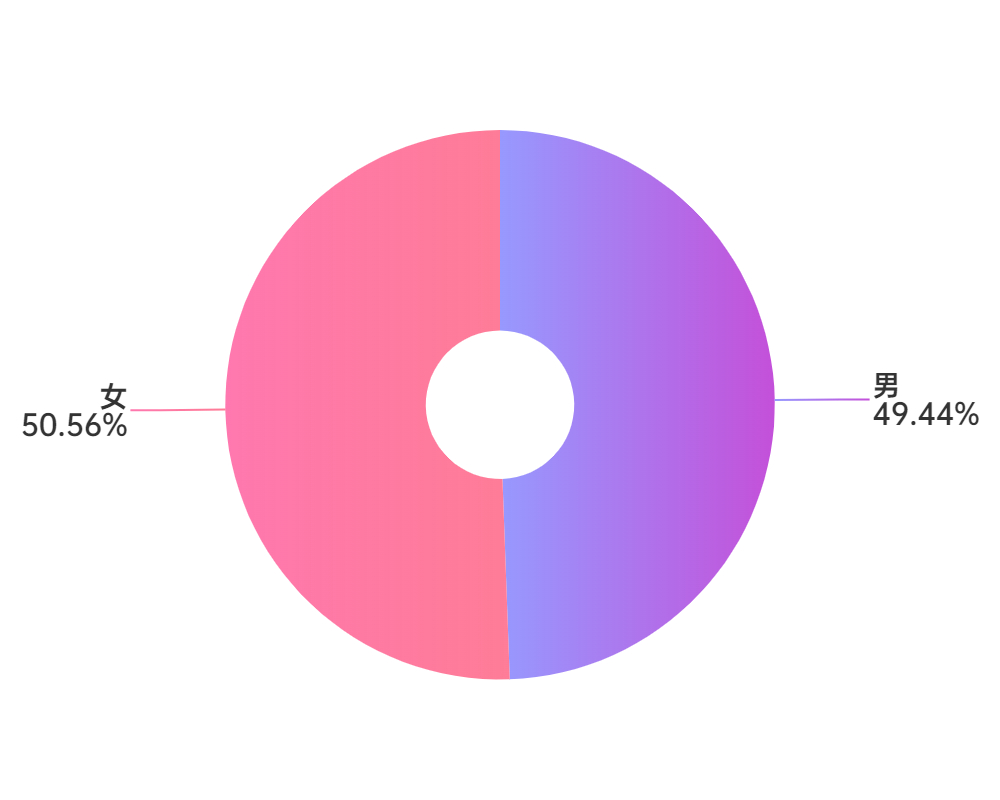
\includegraphics[width=0.4\textwidth]{./pic/性别分布.jpg}}
    \subfigure[年龄分布]{\label{pic:age}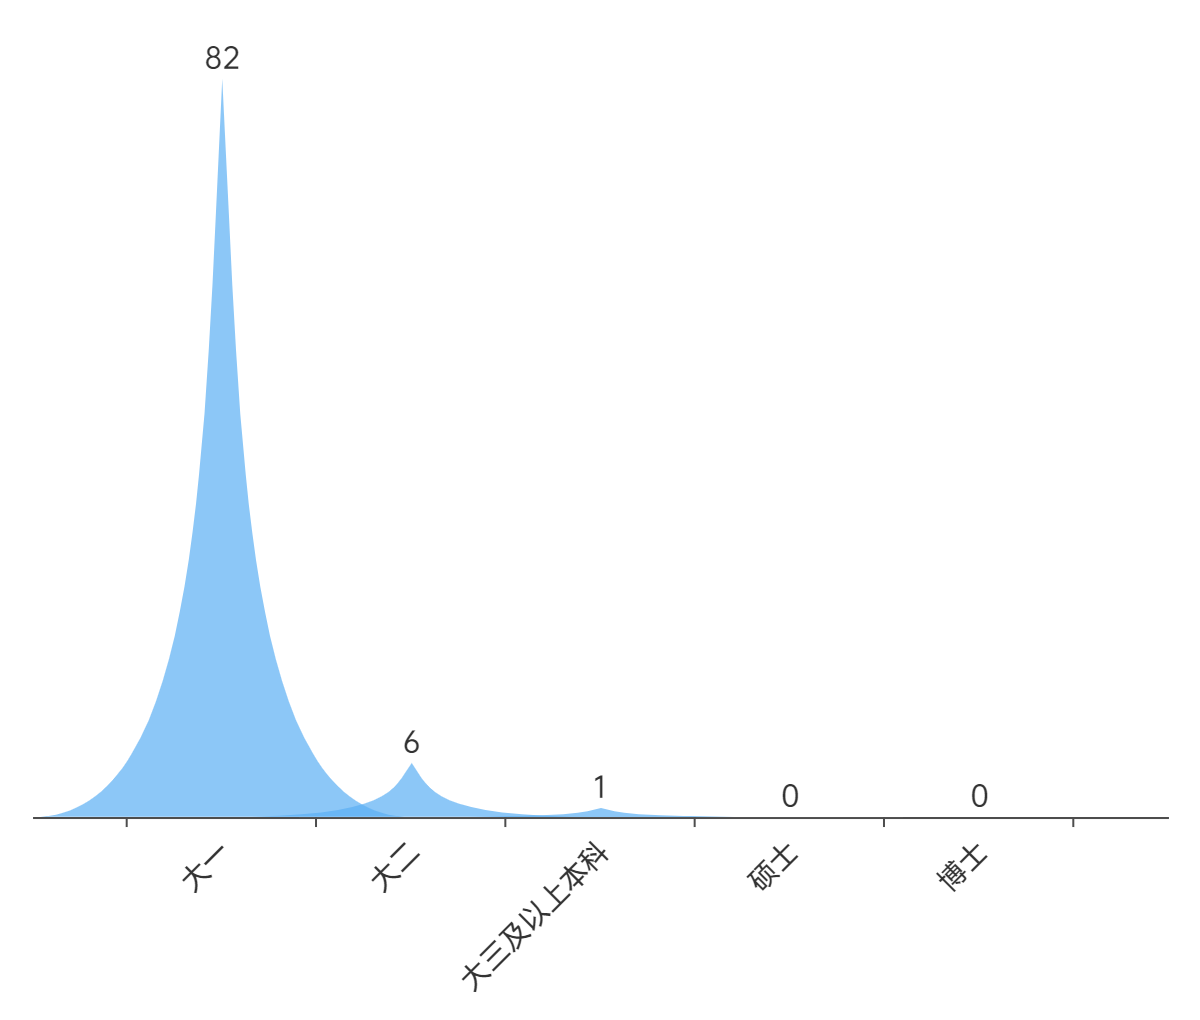
\includegraphics[width=0.4\textwidth]{./pic/年龄分布.png}}
    \caption{样本总体情况概览}
    \label{pic:overall}
\end{figure}

\subsection{对于化妆和医美的看法}
在对化妆和医美的态度上,近一半同学持中立态度,没有特别明显的喜憎表达,如图(\ref{pic:yimei})所示。
\begin{figure}[H]
    \centering
    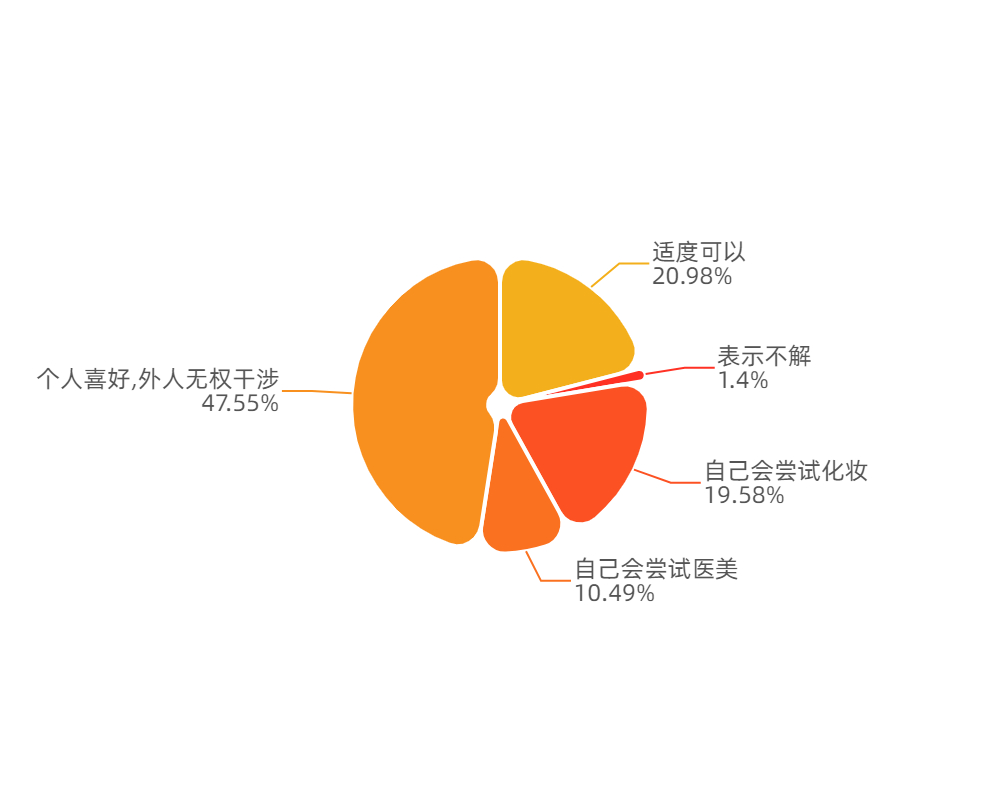
\includegraphics[width=0.4\textwidth]{./pic/对于化妆和医美的看法.jpg}
    \caption{对于化妆和医美的看法}
    \label{pic:yimei}
\end{figure}
\subsection{在整理容貌上花费的时间}
\begin{enumerate}[leftmargin=7em]
    \item 绝大部分同学不会花大量的时间

    根据数据分析,大多数人(93.26\%)每天在修饰自身容貌上花费的时间少于1.5小时,表明大部分人对个人形象的关注和维护是相对合理的。

    仅有4.49\%的人花费1.5小时到3小时,而超过3小时的人更是仅占2.25\%。

    \item 仅极少数同学会花较多时间,且这部分同学中,大部分为女生

    相较于男生群体,女生群体在整理修饰容貌上可能会需要更多的时间,也可能更倾向于在此方面投入较多时间。

\end{enumerate}
\begin{figure}[H]
    \centering
    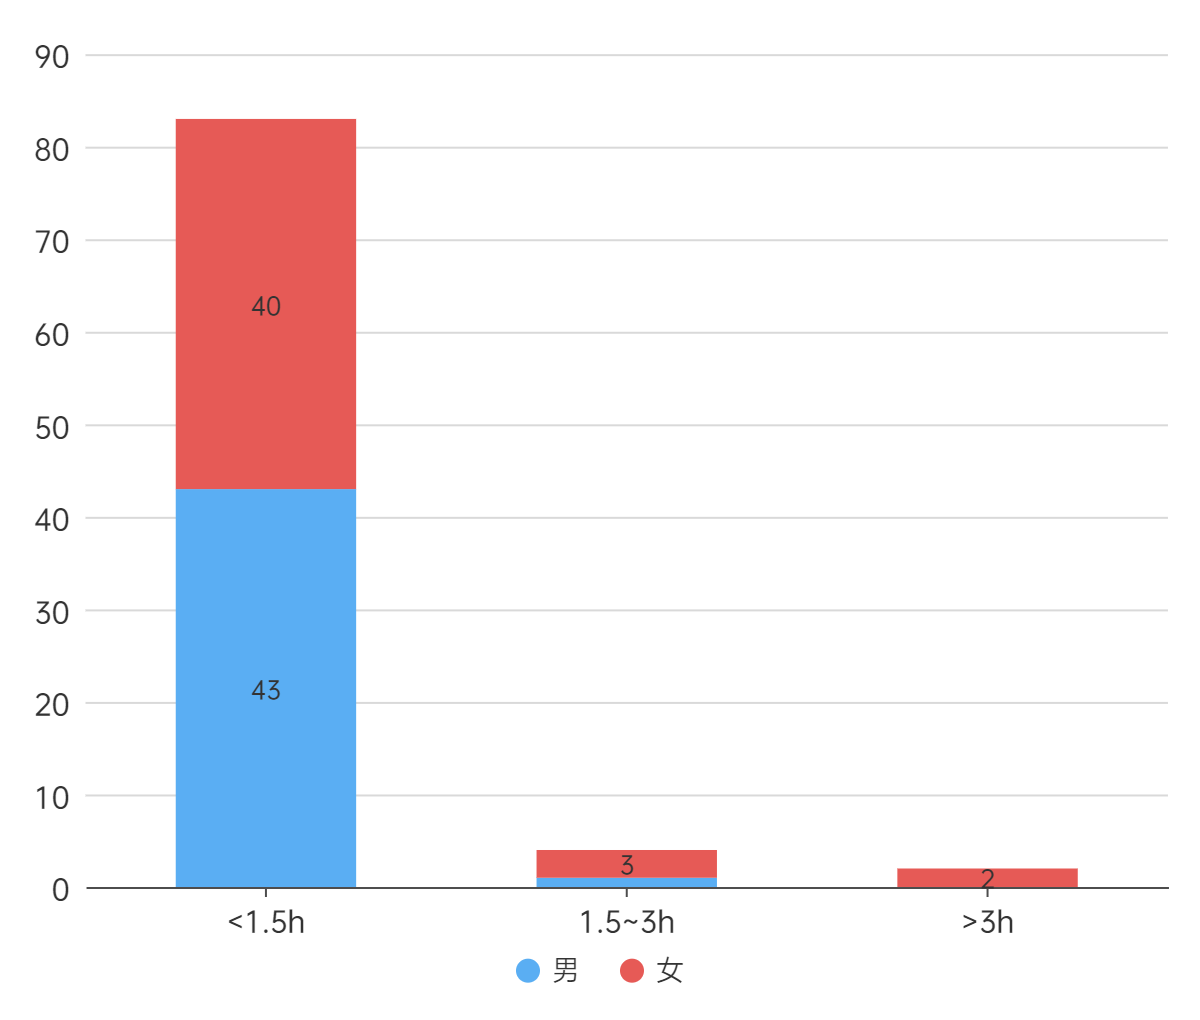
\includegraphics[width=.5\textwidth]{./pic/整理容貌所用的时间.png}
    \caption{整理容貌所用的时间}
    \label{pic:times}
\end{figure}
\subsection{对花时间整理容貌的看法}
\begin{enumerate}[leftmargin=7em]
    \item 大多数被试者(93.26\%)认为整理容貌可以改善精神面貌,
    表明新时期大学生群体大多能正视容貌的价值和作用,并认为外貌与精神状态之间存在一定的正相关关系。

    \item 少数(6.74\%)的被试者认为自己过于关注外貌,受到了负面影响。

    对于这类同学,我们进一步设问关于花费大量时间整理容貌的原因,得出以下结论:
    \begin{enumerate}
        \item 主要原因是\textbf{社会竞争压力增大},劳动力素质普遍得到提高,外在形象对于大学生群体的价值比重有所提升;
        \item 部分\textbf{男生}还认为是\textbf{恋爱}的导致的容貌需求;
        \item 部分\textbf{女生}认为更多的受到了\textbf{医美广告}、\textbf{化妆广告}及\textbf{网红的言论}和\textbf{视频}影响。
    \end{enumerate}
\end{enumerate}
\begin{figure}[H]
    \centering
    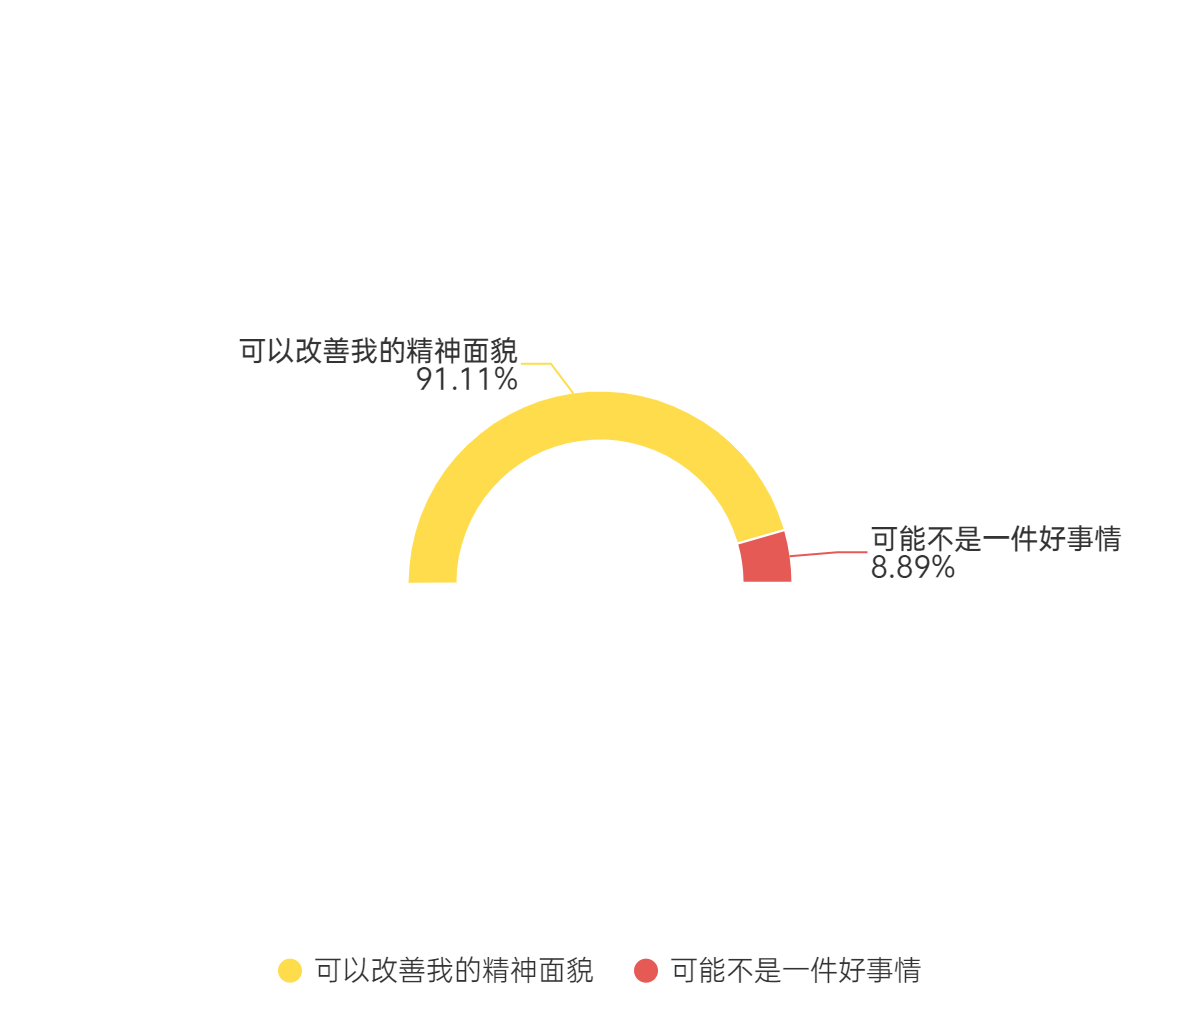
\includegraphics[width=.4\textwidth]{./pic/整理容貌的看法.png}
    \caption{整理容貌的看法}
\end{figure}
\subsection{对容貌焦虑的解决办法及效果}
仅少数同学选择暂时忽略问题,大部分同学选择主动解决,他们表现出积极向好的心态。

大多数表现出容貌焦虑的群体尝试的方法是将关注点转向内在品质,其它解决方法也都取得了不错的效果。
\begin{figure}[H]
    \centering
    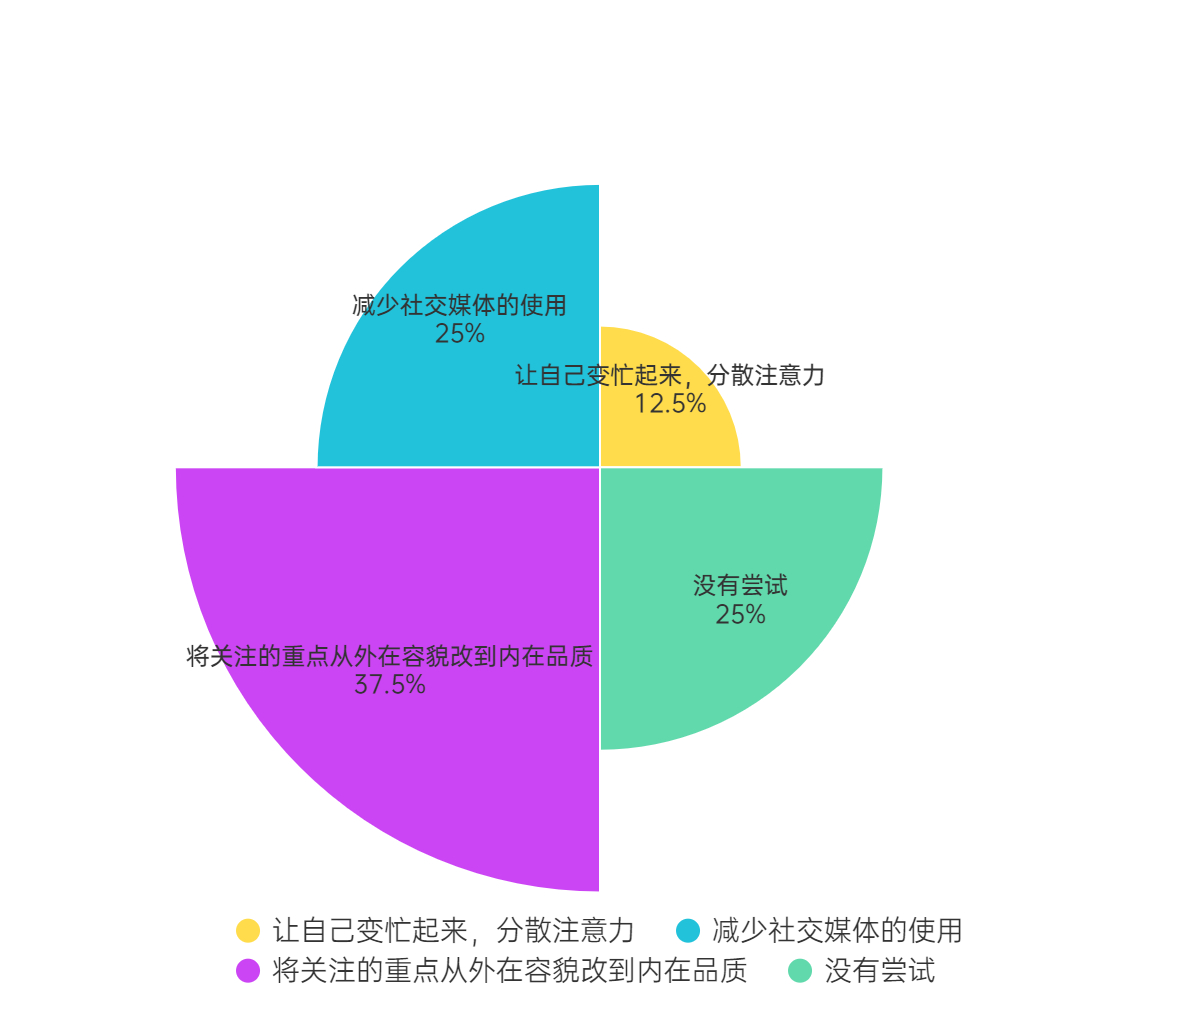
\includegraphics[width=.5\textwidth]{./pic/解决.jpg}
    \caption{对容貌焦虑的解决办法及效果}
\end{figure}
\subsection{总结}
\begin{enumerate}[leftmargin=7em]
    \item 容貌焦虑''现象发生率的性别差异化表现仍然存在,但差异程度有一定的降低。究其原因,可能是因为调查样本主要集中在受教育水平较高且已初步形成较为成熟的价值观的大一学生群体,在自我价值评判体系中,他们会更为重视学识、能力、道德等,也能做到减少外部因素对自身价值观的扭曲。
    \item 大学生群体容貌焦虑的原因主要集中在社会竞争压力上,表明他们可能把面试、面见重要客户这类需要重视容貌的特殊场景过度生活化,同时也有过度抬高容貌在价值体系中的比重的可能,再深入切入也表明大一学生对社会工作认知的切实性不高,其中也可能受到部分影视作品中的戏剧化处理部分的影响,对自我社会竞争力有一定程度上的错误认知。
    \item 大学生群体容貌焦虑的原因还包括美颜技术、医美和化妆品广告及网红宣传以及恋爱的需求,这反映出:部分商家、网红为了利益为``畸形审美''造势,对大学生群体造成了消极影响;部分夸张、悬浮的偶像爱情剧对大学生群体恋爱观的消极影响;大学生容貌焦虑群体在恋爱中一些不愉快体验对他们的恋爱观造成了深刻影响。
    \item 样本中有容貌焦虑表现的大学生群体在日常整理修饰容貌中所花时间并不多,也未表现出明显的想进行医美、化妆的意愿,这也体现出他们的容貌焦虑程度并不高,只是当前一段时间的消极情绪。
    \item 从大一学生群体总体来看,审美健康化已成为主流,他们对容貌的价值认知较为客观理性,遇到问题也多持有积极解决问题的良好心态。
\end{enumerate}

\section{采访内容呈现}
\subsection{采访刘艳老师}
\subsubsection{刘艳老师介绍}
刘艳,女,硕士,讲师,心理中心专职咨询师。中国心理学会临床心理学注册工作委员会注册心理师,国家二级心理咨询师,
国际聚焦取向咨询师(FOT)。16年心理学专业熏陶,13年分析心理学受训,10年人本主义聚焦取向心理学受训。从事心理咨询工作10余年,
个体咨询5000小时以上,团体咨询1000小时以上。
个案类型集中在大学生、儿童青少年与成年女性。
工作风格乃以分析心理学为主的动力学取向,整合沙盘游戏等表达性疗法与聚焦疗法。
\subsubsection{采访节选}
问:您对``容貌焦虑''有哪些了解?

答:``容貌焦虑''并非明确的心理或精神障碍诊断概念,只是社会上的流行说法。它涵盖了人们对外在形象是否符合某种标准的担忧,可实际上根本没有这样的标准。在真实生活中,相处久了,大家不会仅凭容貌定义一个人。但社会上存在一种认知,觉得漂亮很重要,似乎要达到某个不知从何而来的标准。

我遇到过一些情况,有人觉得必须整容,否则大学都读不下去,甚至日子都过不下去。这种``容貌焦虑''是一种外在表现,是担心容貌不够好而失去某些东西。
社会心理学对此有研究,比如韩国整容业发达,是因为在韩国有一种社会认知:长得漂亮意味着拥有其他美好品质,打扮好、长得好的人可能更精明或有更多权力,在事业等方面表现更好,这就像晕轮效应,因外貌给人加上光环。这种社会认知与国家或集体的经济发展水平、社会形态、历史发展阶段都有关系。

在我国,这种现象在21世纪后变得比较夸张,担心容貌影响自身发展只是表象。从我的接触来看,有``容貌焦虑''的人,可能自尊水平很低,无法确定自己不管化不化妆都能被他人接受,所以必须呈现出完美的一面才放心。他们的安全感也可能较差,或许还曾因他人以审视的目光对待自己而受伤,比如社会推崇两米的身高为理想型,很多人达不到,这种社会潮流很容易形成,也很容易用一种社会认知去打击一群人。但每个人的承受能力不同,有的人由于成长经历,没有强大的内心,真的难以承受。

问:如何克服``容貌焦虑''呢?

答:比较简单的方法就像我们刚才提到的,要塑造自己的内核。真正去发现自己的多个方面,要知道自己拥有很多资源。即便没有刻意打扮自己,我们依然可以对自己有良好的感觉。比如说,有一次同学们为我鼓掌,不是因为我化了妆,我甚至都不清楚自己做了什么,但同学们就是喜欢和我在一起。如果这样的经历越来越多,我们就越不需要依靠那些外在的堆砌了。
其实每个人都应该多花些心思在自己身上。现在,我们把太多精力放在关注别人创造的内容上了,比如短视频,却太少进行自我反思,将注意力回归自身。我们已经太久忽略了和自己内心的联系,甚至把这种自我关注看作是无用的,将其价值贬低、功利化。似乎什么都可以被功利化,但这样我们却失去了一些本真的东西。

当我们深入钻研这个话题到一定程度时,其实可以倡导一种新的社会文化。就像之前提到的那种单一的审美标准,比如``两米才是美''这种观念,我们可以推翻它,构建一个多元文化的世界,鼓励每个人更多地关注自身。如果我们去倡导这样的理念,社会会不会因此发生一些改变呢?会不会让那些深受容貌焦虑困扰的人得到解脱呢?我们可以试着把问题反过来思考。

就像我们之前在做女性相关宣传的时候,以一个知名女性内衣品牌为例,在它的广告里,不同高矮、胖瘦、民族、肤色的女性穿上内衣都展现出自信。如果我们多传播这样的信息,有没有可能给社会带来一些积极的改变呢?所以,除了个人要塑造稳定的内核,我们还需要创造不一样的文化,这样才能让更多人摆脱困扰,让大家不再为此担忧。

\subsubsection{总结}
``容貌焦虑'' 并非专业的心理或精神障碍诊断概念,而是社会上流行的说法,其根源在于大众追捧却又虚幻无依据的 ``美貌标准'',人们会担忧自身外在形象不符合这种莫须有的标准,进而产生焦虑。

``容貌焦虑''的起因是多方面的。从个体心理角度看,人类天生具有被认可、被接纳的需求,而在现代社会中,容貌往往被视为获取认可的重要途径之一。尤其是对于那些自尊水平较低、安全感不足的个体,他们更依赖外在的容貌评价来构建自我价值感。

其实,``容貌焦虑''也不过是纸老虎,战胜它很容易。首先要重塑强大的 ``内核'',通过挖掘自身多元价值,珍视那些与容貌无关的被认可时刻,将注意力从外界纷扰回归到内心本真,减少对外在容貌的过度依赖,增强自我认同感。同时,社会需要摒弃单一审美标准这种 ``毒瘤'',构建多元包容的文化,倡导多元美的信息,打破刻板审美禁锢,从整体文化氛围上帮助人们摆脱容貌焦虑的困扰。

\subsection{采访同学}
问:你认为你存在容貌焦虑吗?你是如何判断的?

答:存在。我觉得这是基于一定的水准,内心有着想往更加向善向好的容貌方向发展的渴望,同时也夹杂着一种焦虑感和攀比心理吧。

问:你认为你的这种审美认识是如何产生的呢?

答:可能是源于平时看的一些篮球赛事片段,还有对电影明星形象的印象吧。

采访同学,我们知道了一些同学容貌焦虑的直接诱因,和形成的心理过程。
\begin{figure}[H]
    \centering
    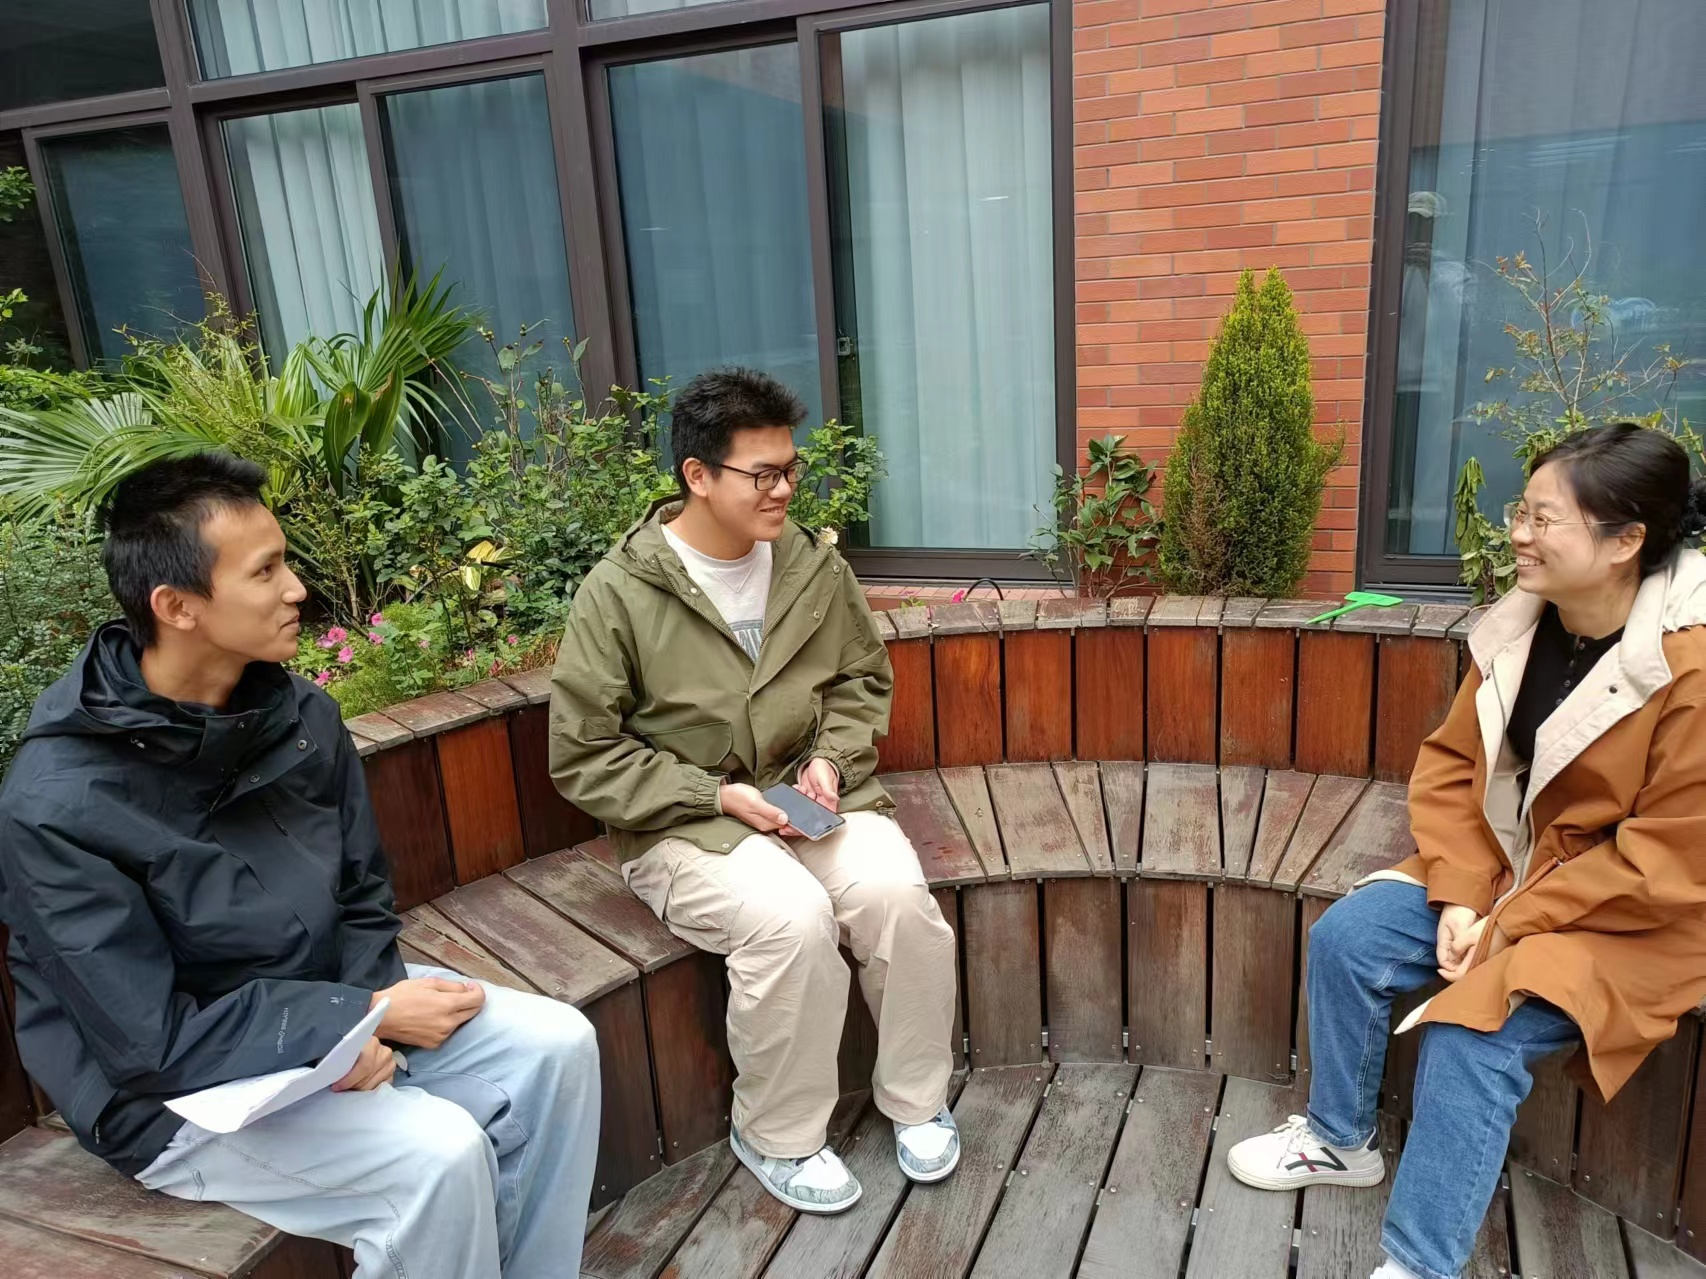
\includegraphics[width=0.7\textwidth]{./assets/采访.jpg}
    \caption{采访图片}
\end{figure}
% \section{医美广告的推动对于容貌焦虑的影响}
% \#TODO
% \input{text/医美广告的推动对于容貌焦虑的影响.tex}
\section{结论}
俄乌冲突既有俄罗斯,乌克兰历史不可调和的矛盾,以及所带来的文化,政治的冲突。
也有西方国家的推波助澜,使得冲突扩大演变为战争。

此次矛盾的核心在于:
\begin{enumerate}
    \item 乌克兰的北约成员国地位问题。
    \item 克里米亚的领土纠纷及乌东地区的独立问题。
    \item 俄罗斯的安全诉求问题。
\end{enumerate}

总体来看,俄乌冲突为世界带来了警示,强调了各国维护和平、坚持国际法和加强外交合作的重要性。

首先,它凸显了地区冲突在全球化时代的深远影响。俄乌冲突不仅局限于两国之间的领土争端,还迅速演变为大国博弈的舞台,导致全球能源和粮食危机,影响了许多国家的经济稳定。

其次,俄乌冲突揭示了国际秩序和规则的重要性。冲突中对主权的侵害、国际法的挑战,以及各国不同的应对措施表明,国际规则的执行和各国对秩序的尊重是维护和平的关键。

此外,俄乌冲突凸显了外交和和平解决争端的必要性。冲突的迅速升级显示出军事手段并不能有效解决深层次的历史和民族矛盾,反而加剧了敌对关系和长期的地区不稳定。和平谈判、外交手段以及对话成为预防战争的最佳途径,避免局部冲突扩大为更严重的全球危机。
\section{参考文献}
\printbibliography[heading=bibliography, title=参考文献]
\newpage
\appendix
{\noindent \Large 附录}
\section{使用AI的感受}
\begin{enumerate}
    \item 何铭源

    `` AI的使用可以简化我的工作,比如信息搜集和信息整理;也可以为我们提供一些创造性的思路。我还在本次的研究性学习中,将不同的课题发送给AI,让他选择一个比较合理的课题。我觉得现在AI的发展大大改善了学生的研究环境,有助于我们更好地进行深度学习。''

    \item 赵皓翌

    ``AI可以在我们指定的一个方向内快速的为我们提供大量的信息,可以节省我们很多的时间,并且在提供信息的同时还给我们提供很多创造性的思维。 ''

    \item 余文乐

    ``使用AI非常的方便,提出问题后,他就可以在短时间内给我提供大量的思路,体验感受非常不错。''

\end{enumerate}
\section{分工安排}
\begin{table}[H]
    \centering
    \caption{分工一览表(排名不分先后)}
    \begin{tabularx}{0.8\textwidth}{>{\raggedright\arraybackslash}X
        | >{\raggedright\arraybackslash}X}
        \hline
        \textbf{组员} & \textbf{工作}                                             \\ \hline
        郭慧婷         & 提出总课题方向,撰写课题详述、研究思路、研究方法、问卷大纲、数据分析结论和研究总结文本,参与查找相关论文,参与制作结题PPT,并进行了校对和展示,校对研究性报告,组织小组进行讨论。           \\ \hline
        何铭源         & 研究现状文献整理、问卷大纲撰写、综合整理研究数据及采访资料,帮助整理小组结论、开题结题PPT制作、结题报告撰写 \\ \hline
        蒋子墨         & 整理研究现状、参与了问卷问题的拟定、采访心理老师                                \\ \hline
        阎乐暄         & 整理研究现状、参与问卷调查问题的讨论与拟定、结题前分析论文并进行总结归纳                    \\ \hline
        诸葛一涵        & 整理研究现状、参与了问题的拟定、采访了一位同学并录音、在结题前参考文献资料并提出了一些观点           \\ \hline
        江善钊         & 整理了研究现状、参与设计问卷、回收问卷数据并对数据进行了可视化                         \\ \hline
        任弈          & 对``容貌焦虑''进行概念界定、采访记录并总结                                   \\ \hline
        赵皓翌         & 参与问卷调查问题的讨论和拟定、结题前对论文进行分析                               \\ \hline
        余文乐         & 参与制作开题PPT框架、参与问卷调查问题的讨论与拟定、采访相关老师、结题前分析论文并进行总结归纳       \\ \hline
    \end{tabularx}
\end{table}
\newpage
\section{问卷全文}
\subsection{调查结果}
通过发布问卷,我们初步调查了大学生信息收集的现状,得到的结果如下:
\begin{enumerate}
    \item \textbf{主要年龄段}:受调查的群体主要集中在18–22岁,占90.91\%。
    \item \textbf{主要获取信息的平台}:视频平台和搜索引擎是大学生主要的信息获取渠道,分别占36.36\%和30.91\%,这表明大学生更倾向于使用便捷且信息丰富的平台来获取信息。然而,这也从某种程度上体现出大学生在搜索时不太注重结果的可信度,尤其是视频平台的信息繁杂且难以准确检索。
    \item \textbf{信息搜索的内容}:学习相关的信息搜索占比最高,达90.91\%,这与大学生的主要任务相符合。生活困惑、活动信息等也是大学生常搜索的内容。
    \item \textbf{信息搜索的习惯}:80\%的大学生在解决问题时习惯先搜索,这说明他们在面对问题时更倾向于主动获取信息来解决。
    \item \textbf{信息搜索能力的评价}:超过半数的大学生认为自己的信息搜索能力足够,但仍有45.45\%的人认为不够,这表明部分同学在此方面还有提升空间。
    \item \textbf{信息检索能力对生活的影响}:绝大多数大学生认为信息检索能力对日常学习生活有显著影响,占比90.91\%,凸显了提高该能力的重要性。
    \item \textbf{信息检索能力不足的原因}:数据显示,缺乏检索知识及相关技能是主要原因(92\%),此外,缺少相关课程(56\%)和对设备操作不熟悉(52\%)也是重要因素;电子文盲现象普遍,许多同学在大学前未系统学习电脑操作,进一步制约了检索能力。
    \item \textbf{提高信息检索能力的方式}:开设信息素养课程(80\%)、举办信息素养讲座与培训(74\%)和参加信息实践活动(76\%)是大学生认为最有效的提升途径。
    \item \textbf{信息检索技巧的掌握情况}:只有38.18\%的大学生表示掌握一些检索技巧,多数人对技巧的了解仍较有限。
    \item \textbf{检索结果的相关性}:近一半的大学生经常遇到无法检索到理想结果或仅检索到弱相关结果的情况,说明检索精准度有待提高。
    \item \textbf{搜索结果的筛选方式}:大部分大学生会根据关键字吻合度来筛选结果(87.27\%),同时也会参考热度数据和过来人的评论。
\end{enumerate}
\subsection{拟解决方法}
根据以上调查结果,我们组思考出一下解决方法:
\begin{ffbox}{开设信息素养课程}{}

学校可以开设专门的信息素养课程,系统地教授信息检索知识和技能,如布尔逻辑检索、截词检索等技巧,以及如何使用不同的数据库和搜索引擎。对于数据库检索能力的提升尤其有必要,目前数据库是储存许多专业信息的重要形式,但许多同学甚至没有听说过数据库检索,也没有了解过一些实用的数据库。
\end{ffbox}

\begin{ffbox}{举办信息素养讲座与培训}{lecture}

学校可以邀请专业人员开展信息素养讲座和培训,介绍最新的检索工具和方法,提高大学生的信息检索意识和能力。
\end{ffbox}

\begin{ffbox}{参加信息实践活动}{comp}

组织大学生参与信息检索相关的实践活动,如信息检索比赛、科研项目中的文献检索等,增加实际操作经验。
\end{ffbox}

\begin{ffbox}{注重检索技巧的学习}{study}

大学生应主动学习和掌握各种信息检索技巧,提高检索效率和准确性。
\end{ffbox}

\begin{ffbox}{优化信息筛选方法}{}

除了根据关键字吻合度筛选结果外,还应学会结合来源可靠性、信息权威性等多种因素综合判断,提高信息质量。
\end{ffbox}
根据实践的难易程度,我们组选择进行\nameref{way:lecture}与\nameref{way:comp}作为主要活动。
\newpage
\section{采访全文}
在这个信息过载的时代,检索能力已成为核心学术竞争力之一。
我们的采访所揭示的,不仅是个体的困惑,更是整个教育体系需要应对的时代命题。
我们不仅需要专业知识,更需要在大浪淘沙的信息海洋中辨别真伪、提取精华的能力。

\subsection{实操困境}
当被问及课程论文写作的第一反应时,学术数据库成为首选,这反应出我们的学生虽然知道应该使用正规学术渠道,却在实操层面面临诸多困境:
关键词搜索成为横亘在学术探索道路上的一道障碍。
"不确定自己搜的关键词对不对"、
"专业术语让人迷惑"等反馈\dots

学术数据库的检索逻辑与日常搜索引擎大相径庭、
但鲜有课程系统教学这一关键技能。
更值得玩味的是,受访者提到的"把中文关键词机翻成英文再搜索"的小技巧,
既展现了学生的创造性,也折射出工具使用教育的不足——这本应是基础技能,却成了需要自行摸索的"技巧"。

\subsection{信息渠道多元化}
值得指出的是,信息获取渠道的多元化趋势在采访中尤为明显。
短视频平台、校园论坛、经验分享会与传统学术数据库共同构成了学生的信息来源。
学生对学长学姐经验的重视反映出学术界一个长久存在的困境:隐性知识的传承往往依赖于非正式渠道。
同时,AI工具的崛起正在重塑信息检索的生态。学生对"用AI工具快速筛选文献"的强烈需求,既是对效率的追求,也隐含对传统检索方式的不满。
但关键在于,我们需要明白如何与AI协作而非依赖,如何用批判性思维审视AI提供的结果,而非全盘接受。


\end{document}